\chapter{Metoda končnih elementov}\label{sec:MKE}
    
    Ker ima realni metamaterial v resnici končno število reprezentativnih celic in ker so te za analitično reševanje preveč kompleksne, bomo njegovo dinamiko rešili z uporabo metode končnih elementov (MKE). V poglavju \ref{sec:meritev_materialnih_lastnosti} uporabimo MKE v povezavi z eksperimentalnimi meritvami tudi za določitev modula elastičnosti $E$ osnovnega materiala.
    
    MKE je iskanje rešitev kompleksnega realnega problema z uporabo poenostavljenega modela, ki sestoji iz številnih delov, imenovanih končni elementi (KE). Torej zvezno območje diskretiziramo v podobmočja, zato je MKE po naravi aproksimativna metoda in je uporabna takrat, kadar analitična rešitev ni mogoča.
    
    Neodvisno od geometrije in celo od vrste fizikalnega problema, ki ga želimo rešiti z MKE, so osnovni koraki formulacije vedno enaki. Preko njih bomo na osnovi pregleda literature \cite{rao2010theFEMinEngineering} izpeljali enačbe MKE in reševali dinamsko analizo lastnih nihanj DVA-ja. 
    
    \textbf{Korak 1:} Razdelitev fizikalnega modela v diskretne elemente (diskretizacija).\smallskip\newline
    Na tem mestu izberemo tip, število in velikost KE. Problem bomo reševali z splošnimi volumskimi heksaedričnimi KE. 
            
    \textbf{Korak 2:} Izbira aproksimacijskega modela.\smallskip\newline
    Izberemo obliko poljubne aproksimacijske funkcije, ki določa aproksimacijo primarne spremenljivke. Najpogosteje gre za polinomske funkcije.

    \textbf{Korak 3:} Izpeljava matrik končnega elementa.\smallskip\newline
    Za KE v svojem lokalnem koordinatnem sistemu (KS) diferencialno enačbo fizikalnega problema zapišemo kot integralsko variacijsko formulacijo. Uporabimo prej izbrano interpolacijsko funkcijo in dobimo značilne matrike sistema v lokalnem KS. Sledi transformacija koordinat v globalne matrike. 

    \textbf{Korak 4:} Sestavljanje matrik posameznega končnega elementa v sistemske matrike.\smallskip\newline
    Matrike posameznih elementov razširimo na vse prostostne stopnje in jih seštejemo.

    \textbf{Korak 5:} Upoštevanje začetnih pogojev ter robnih in prehodnih pogojev.

    \textbf{Korak 6:} Reševanje sistema enačb.
    
    Definirajmo sedaj gibalne enačbe končnega elementa za reševanje problema lastnih nihanj in jih kasneje aplicirajmo na oba uporabljena tipa končnih elementov. 

    \newpage
    \section{Gibalne enačbe končnega elementa}
    
        Pomike po območju končnega elementa $\vv U$, aproksimiramo preko diskretnih vrednosti pomikov vozlišč $\vv{Q}^e$ in matrike oblikovnih oziroma aproksimacijskih funkcij $[N]$: 
        \begin{equation}\label{eq:KE_polje_pomikov}
            \vec{U}(x, y, z, t)=\left\{\begin{array}{l}
            u(x, y, z, t) \\
            v(x, y, z, t) \\
            w(x, y, z, t)
            \end{array}\right\}=[N(x, y, z)] \vv{Q}^e(t)\,.
        \end{equation}
        Za KE lahko izrazimo specifične deformacije $\vv \epsilon$ in napetosti $\vv \sigma$:
        \begin{align}
            \vv{\varepsilon}&=[B] \vv{Q}^e \label{eq:KE_deformacije} \,, \\
            \vv{\sigma}&=[D] \vv{\varepsilon}=[D][B] \vv{Q}^e, \label{eq:KE_napetosti}
        \end{align}
        kjer je $[B]$ matrika odvodov oblikovnih funkcij in $[D]$ materialna matrika, v kateri se nahaja modul elastičnosti. Z odvajanjem enačbe \eqref{eq:KE_polje_pomikov} po času definiramo polje pomikov, kjer je $\dot{\vv{Q}^e}$ diskretna vrednost vozliščnih hitrosti:
        \begin{equation}
            \dot{\vv{U}}(x, y, z, t)=[N(x, y, z)] \dot{\vv{Q}^e}(t)\,.
        \end{equation}
        Gibalne enačbe izpeljemo preko Lagrangeve formulacije:
        \begin{equation}\label{eq:KE_Lagrange}
            \frac{\mathrm{d}}{\mathrm{d} t}\left\{\frac{\partial \mathcal{L}}{\partial \dot{Q}}\right\}-\left\{\frac{\partial \mathcal{L}}{\partial Q}\right\}+\left\{\frac{\partial E_d}{\partial \dot{Q}}\right\}=\{0\} \,,
        \end{equation}
        kjer je Lagrangian $\mathcal{L}$ definiran z razliko kinetične $E_k$ in potencialne $E_p$ energije. Za vsak element lahko kinetično, potencialno in disipacijsko energijo zapišemo kot $E_d$:
        \begin{align}
            E_k^e&=\frac{1}{2} \iiint_{V^e} \rho \dot{\vv U}^{\text{T}} \dot{\vv U} \mathrm{~d} V \,,\\
            E_p^e&=\frac{1}{2} \iiint_{V^e} \vv{\varepsilon}^{\text{T}} \vv{\sigma} \mathrm{d} V-\iint_{S^{e}} \vv{U}^{\text{T}} \vv{\overline{\Phi}} \mathrm{d} S -\iiint_{V^e} \vv{U}^{\text{T}} \vv{\overline{\phi}} \mathrm{d} V \,,\\
            E_d^e&=\frac{1}{2} \iiint_{V^{e}} c \vv{U}^{\text{T}} \dot{\vv{U}} \mathrm{~d} V \, . 
        \end{align}
        Pri tem je $\rho$ gostota in $c$ koeficient dušenja. $\vv{\overline{\Phi}}$ je vektor sil na zunanjih površinah in $ \vv{\overline{\phi}}$ vektor sil kot posledica volumskih obremenitev  elementa. 
        Seštejemo energije po posameznih elementih:
        \begin{align}
            E_k=\sum_{e=1}^{E} E_k^{e}&=\frac{1}{2} \vv{Q}^{\text{T}}\left[\sum_{e=1}^{E} \iiint_{V^e} \rho[N]^{\text{T}}[N] \mathrm{d} V\right] \dot{\vv{Q}} \,,\\
            E_p=\sum_{e=1}^{E} E_p^{e}&=\frac{1}{2} \vv{Q}^{\text{T}}\left[\sum_{e=1}^{E} \iiint_{V^e}[B]^{\text{T}}[D][B] \mathrm{d} V\right] \vv{Q} \nonumber \\ 
            &-\vv{Q}^{\text{T}}\left(\sum_{e=1}^{E} \iint_{S^{e}}[N]^{\text{T}} \vec{\Phi}(t) \mathrm{d} S^e+\iiint_{V^e}[N]^{\text{T}} \vv{\overline{\phi}}(t) \mathrm{d} V\right)-\vv{Q}^{\text{T}} \vv{F_c}(t) \,,\\
            E_d=\sum_{e=1}^{E} E_d^{e}&=\frac{1}{2} \vv{Q}^{\text{T}}\left[\sum_{e=1}^{E} \iiint_{V^{(e)}} c[N]^{\text{T}}[N] \mathrm{d} V\right] \dot{\vv{Q}} \,.
        \end{align}
        Pri tem so $\vv{Q}$ globalni vektor vozliščnih pomikov, $\dot{\vv{Q}}$ hitrosti in $\vv F_c$ vektor koncentriranih vozliščnih sil. Iz zgornjih izrazov lahko razberemo masno $[M^e]$, togostno $[K^e]$ in disipacijsko $[C^e]$ matriko posameznega elementa in vektor ekvivalentnih vozliščnih sil zaradi površinskih učinkov $ \vv F_S^e$ ter zaradi volumskih učinkov $ \vv F_V^e$:
        \begin{align}
            \left[M^{e}\right]&=\iiint_{V^e} \rho[N]^{\text{T}}[N] \mathrm{d} V \label{eq:M_matrika} \,, \\
            \left[K^{e}\right]&=\iiint_{V^e} [B]^{\text{T}}[D][B] \mathrm{d} V \label{eq:K_matrika} \,, \\
            \left[C^{e}\right]&=\iiint_{V^e} c[N]^{\text{T}}[N] \mathrm{d} V \,, \\
            \vv F_S^e&=\iint_{S^{e}}[N]^{\text{T}} \vv{\overline{\Phi}} \cdot \mathrm{d} S \,, \\
            \vv F_V^e&=\iint_{V^{e}}[N]^{\text{T}} \vv{\overline{\phi}} \cdot \mathrm{d} V \,.
        \end{align}
        Če lokalne matrike razširimo na vse prostostne stopnje in jih seštejemo dobimo masno $[M]$, togostno $[K]$ in disipacijsko $[C]$ matriko celotnega sistema. Seštevek vseh ekvivalentnih vozliščnih vrednosti sil po vseh elementih $F_S^e$ in $F_V^e$  in dodatni prispevek vseh koncentriranih vozliščnih vrednosti nam vrne globalni vektor vozliščnih sil $\vv F(t)$. Definicijo masne, togostne in disipacijske matrike upoštevamo pri energijskih izrazih, ki jih vstavimo v enačbo \eqref{eq:KE_Lagrange} in dobimo globalni sistem gibalnih enačb pridobljen z metodo končnih elementov, pri čemer je $\ddot{\vv{Q}}$ vektor globalnih vozliščnih pospeškov:
        \begin{equation}
            [M] \ddot{\vv{Q}}(t)+[C] \dot{\vv{Q}}(t)+[K] \vv{Q}(t)=\vv{F}(t) \,.
        \end{equation}
        V nadaljnji obravnavi lahko zanemarimo dušenje:
        \begin{equation}\label{eq:KE_final}
            [M] \ddot{\vv{Q}}(t)+ [K] \vv{Q}(t)=\vv{F}(t) \,.
        \end{equation}

    \section{Statična analiza pri velikih pomikih}

        Če želimo ovrednotiti nelinearne učinke KNT vzmeti poglavja \ref{sec:ROC_statika} z uporabo MKE, moramo razumeti, da obstajajo tri vrste nelinearnosti, ki jih moramo upoštevati. Materialne nelinearnosti so potrebne za napovedovanje plastičnih deformacij. Kontaktne nelinearnosti so potrebne za napovedovanje spremembe stanja in drsnega trenja med sestavnimi deli. Tretja možnost, geometrijska nelinearnost, vključuje spremembe geometrije, ki vodijo v povečanje togosti. Povzeto po \cite{Crisfield2000}.

        V enačbi \eqref{eq:KE_deformacije} smo specifične deformacije definirali kot linearne funkcije diskretnih vrednosti pomikov vozlišč $\vec Q^e$. Pri velikih pomikih ne moramo predpostaviti linearne odvisnosti deformacije. Postopamo tako, da je togost $[K]$ enačbe \eqref{eq:KE_final} funkcija pomika, zanemarimo pa tudi $[M]$:
        \begin{equation}
            [K(\vv Q)] \, \vv{Q}=\vv{F} \,.
        \end{equation}

        Ker je numerično reševanje nelinearnega problema kompleksno, postopamo tako, da rešujemo iterativno in ob vsakem časovnem koraku primerjamo linearno togost $[K]$ pridobljeno iz statičnega ravnovesja sil enačbe \eqref{eq:KE_final}  in posodobimo geometrijo. 

        
    \newpage
    \section{Analiza lastnih nihanj}\label{sec: AnalizaLastNihanj}
        Poljubnemu sistemu lahko v začetku opazovanja dodelimo neke začetne pogoje, nato pa mu prepustimo, da prosto niha. Po vnosu začetnih pogojev struktura ni pod vplivom nobene zunanje sile in pravimo, da je sistem v stanju proste vibracije  \cite{boltezar2010mehanska}.
        Matematični izhodišče pri iskanju lastnih frekvenc (lastnih vrednosti) in pripadajočih lastnih oblik predstavlja enačba \eqref{eq:KE_final}, pri čemer je $\vv F=0$:
        \begin{equation}\label{eq:gib_en_lastna}
            [M] \ddot{\vv{Q}}+[K] \vv{Q}=\vv 0\,.
        \end{equation}
        Gre za sistem $n$ homogenih gibalnih enačb, kjer je $n$ število prostostnih stopenj. Za nedušene in harmonične proste vibracije iščemo rešitev kot $n$ harmonskih funkcij zapisanih v vektorski notaciji kot:
        \begin{equation} \label{eq:harmonska_funkcija}
            \vv Q= \vv{\overline{Q}} \, e^{i \omega t} \,,
        \end{equation}
        kjer so iskane neznane vrednosti amplitude $\vv{\overline{Q}}$ in lastne frekvence $\omega$. Sistem ima $n$ lastnih frekvenc ter enako število lastnih oblik.
        Nastavek \eqref{eq:harmonska_funkcija} uporabimo v enačbi \eqref{eq:gib_en_lastna}:
        \begin{align}\label{eq:karakteristica_en}
            -\omega^2 [M]\ddot{\vv{Q}} \, e^{i \omega t}+[K]\vv{Q} \,e^{i \omega t}&=\vv 0 \, \textrm{ / predp. } \,e^{i \omega t} \neq 0\nonumber \,, \\
            \left(\,[K]-\omega^2[M] \, \right) \vv{\overline{Q}}&=\vv 0 \, \textrm{ / pomnožimo z }[M^{-1}]\nonumber \,, \\
            \left(\,[A\,]-\lambda \, [\,I\,] \, \right) \vv{\overline{Q}}&=\vv 0 \,,
        \end{align}
        kjer je matrika $[A\,]=[K][M^{-1}]$ imenovana dinamska matrika sistema. $\lambda=\omega^2$ je parameter, ki vodi do lastnih vrednosti sistema. Netrivialna rešitev zahteva vsaj eno neničelno amplitudo v vektorju $\vv{\overline{Q}}$, torej iščemo neničelnost determinante ali karakteristično enačbo sistema:
        \begin{equation}
            \det \left( \, [A\,]-\lambda \, [\,I\,] \, \right)=0 \,,
        \end{equation}
        Razvoj determinante pripelje do polinoma $n$-te stopnje:
        \begin{equation}
            \lambda^{n}+X_1\lambda^{n-1}+...+X_n=0\text{ ,}
        \end{equation}
        iz katerega izrazimo $n$ lastnih vrednosti sistema. Lastne vrednosti uredimo po velikosti $\lambda_i$, $i=1, ..., n$, tako da najmanjše število pomeni prva lastna vrednost in hkrati prva lastna frekvenca $f_0$:
        \begin{equation}\label{eq:lastna_frekvenca}
            f_{0,i}=\frac{\omega_{i}}{2 \pi}=\frac{\sqrt{\lambda_i}}{2 \pi} \, \textrm{; } i=1,\, ...\,,\,n \,.
        \end{equation}
        Z vstavljanjem izračunanih lastnih vrednosti $\lambda_i$ v enačbo \eqref{eq:karakteristica_en} izračunamo pripadajoče lastne vektorje $\overline{Q}_i$. Lastni vektorji ne predstavljajo dejanske amplitude, temveč medsebojno relativne vrednosti. Če te relativne vrednosti normiramo in formuliramo v vektor $\vv{\overline{Q}}$, ta predstavlja modalno obliko pripadajoče lastne frekvence. 
        V sistemu z velikim številom matrik (v resnici že pri $3 \times 3$ matriki) postane postopek iskanja lastnih vrednosti analitično težko rešljiv. Lastne vrednosti in pripadajoče lastne vektorje iščemo numerično. Numerične metoda hkrati vrnejo sezname lastnih vrednosti $\lambda$ ter seznam desnih normiranih lastnih vektorjev $\vv{\overline{Q}}$. 
        
    \newpage
    \section{Masna in togostna matrika končnih elementov}
        
        V izpeljavi dinamičnih enačb po metodi končnih elementov vidimo, da potrebujemo določiti masno in togostno matriko končnega elementa. Natančno geometrijo metamateriala popišemo z heksaedričnimi volumskimi KE. Te tvori osem vozlišč $i=1\text{-}8$, katerega vsako ima tri prostostne stopnje $u_i$, $v_i$, $w_i$. Izpeljavo izvedemo za izoparametrični KE, tako da je element v naravnem koordinatnem sistemu (KS) $r$, $s$, $t$ vedno kocka (slika \ref{fig:heksaedricni_KE}). Preko Jakobijeve matrike $[J]$ lahko izpeljavo v naravnem transformiramo v kartezijev KS. Velja, da lahko zaradi fizike ponekod problem obravnavamo poenostavljeno. Takrat lahko matrike poenostavimo na dvodimenzionalne. 
        \begin{figure}[!hb]
            \centering
            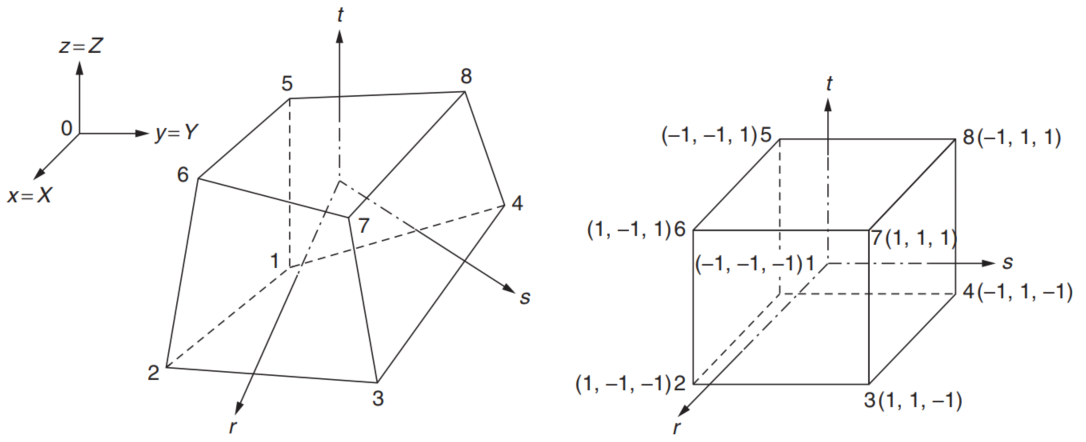
\includegraphics[scale=0.65]{slike/teorija/heksaedricni_KE.png}
            \caption{Heksaedrični KE v kartezijevem (levo) in naravnem (desno) KS \cite{rao2010theFEMinEngineering}. }\label{fig:heksaedricni_KE}
        \end{figure}
        
        Enačbi za masno matriko pridobljeno z \eqref{eq:M_matrika} in togostno matriko z \eqref{eq:K_matrika} se v primeru izoparametričnega heksaerdičnega KE glasita:
        \begin{align}
            \left[M^{e}\right]&=\int_{-1}^{1}\int_{-1}^{1}\int_{-1}^{1} 
            \rho \, ([J]^{-1}[N])^{\text{T}}([J]^{-1}[N]) \, \operatorname{det}[J] 
            \, \mathrm{d} r\, \mathrm{d} s\, \mathrm{d} t \,, \\
            \left[K^{e}\right]&=\int_{-1}^{1}\int_{-1}^{1}\int_{-1}^{1}
            ([J]^{-1}[B])^{\text{T}}[D]([J]^{-1}[B]) \, \operatorname{det}[J] 
            \, \mathrm{d} r\, \mathrm{d} s\, \mathrm{d} t \,,
        \end{align}
        
        kjer je matrika oblikovnih funkcij v naravnem KS: 
        \begin{align}
        &[N]=\left[\begin{array}{cccccc}
        N_{1} & 0 & 0 & N_{2} & \ldots & 0 \\
        0 & N_{1} & 0 & 0 & \ldots & 0 \\
        0 & 0 & N_{1} & 0 & \ldots & N_{8}
        \end{array}\right] \,, \\
        &N_{i}(r, s, t)=\frac{1}{8}\left(1+m_{i}\right)\left(1+s s_{i}\right)\left(1+t t_{i}\right) ; \quad i=1,\,2, \ldots, 8 
        \end{align}
        in matrika odvodov oblikovnih funkcij, ki je dimenzije $6$ x $24$:
        \begin{equation}
        [B]=\left[\left[B_{1}\right]\left[B_{2}\right] \ldots\left[B_{8}\right]\right] \,.
        \end{equation}
        Jakbijeva matrika je definirana kot:
        \begin{equation}
        [J]=
        \left[\begin{array}{ccc}
        \sum_{i=1}^{8}\left(\frac{\partial N_{i}}{\partial r} x_{i}\right) & \sum_{i=1}^{8}\left(\frac{\partial N_{i}}{\partial r} y_{i}\right) & \sum_{i=1}^{8}\left(\frac{\partial N_{i}}{\partial r} z_{i}\right) \\
        \sum_{i=1}^{8}\left(\frac{\partial N_{i}}{\partial s} x_{i}\right) & \sum_{i=1}^{8}\left(\frac{\partial N_{i}}{\partial s} y_{i}\right) & \sum_{i=1}^{8}\left(\frac{\partial N_{i}}{\partial s} z_{i}\right) \\
        \sum_{i=1}^{8}\left(\frac{\partial N_{i}}{\partial t} x_{i}\right) & \sum_{i=1}^{8}\left(\frac{\partial N_{i}}{\partial t} y_{i}\right) & \sum_{i=1}^{8}\left(\frac{\partial N_{i}}{\partial t} z_{i}\right)
        \end{array}\right].
        \end{equation}
        
        
       
       
       
        